\documentclass[10pt]{beamer}

\usetheme{McMaster}
\usepackage{math}

%===Specific for this talk===%
\usepackage{algorithm,algorithmicx,algpseudocode}
\DeclareMathOperator{\iaa}{IAA} % paper specific
\newtheorem{proposition}{Proposition}
\newcommand{\vecw}{\left ( \vec{w}_i^n \right )^\top}
\newcommand{\Aij}{\left ( \hat{A} + E_{i \to j}^{n} \right )^{-1}}
\newcommand{\AijE}{\Aij E_{i \to j}^{n}}
\DeclareMathOperator{\Span}{span}
\DeclareMathOperator{\argmin}{argmin}
\usepackage{tikz, pgfplots}
\usepackage{tikz-3dplot}
\usetikzlibrary{decorations.pathreplacing,positioning,calc,intersections,3d,shapes.geometric,shapes,chains,math,fit,backgrounds}

\tikzset{
	pics/starred/.style={code={
		\filldraw[magenta] (0,0) -- (0,1) -- (1,1) -- (1,0) -- cycle;
		\filldraw[black, opacity=0.2] (0,1) -- (1,0) -- (0,0) -- cycle;
		\filldraw[black, opacity=0.4] (0,0) -- (1,1) -- (0,1) -- cycle;
%		\filldraw[red] (0,0) -- (0.5,0.5) -- (0,1) -- cycle;
%		\filldraw[blue] (0,1) -- (0.5,0.5) -- (1,1) -- cycle;
%		\filldraw[green] (1,1) -- (0.5,0.5) -- (1,0) -- cycle;
%		\filldraw[yellow] (1,0) -- (0.5,0.5) -- (0,0) -- cycle;
%		\filldraw[black, opacity=0.3] (1,0) -- (1,1) -- (0.5,1) -- (0.5,0) -- cycle;
%		\node[star, fill=magenta!30!black] at (0.5,0.5) {};
	}}
}

%===School colours===%
\definecolor{MacMaroon}{HTML}{7A003C} % Primary (dark)
\definecolor{UnigePink}{RGB}{207,0,99}
\definecolor{UnigeGreen}{RGB}{0,126,100}
\definecolor{SFURed}{HTML}{CC0633}
\definecolor{SFUDarkRed}{HTML}{A6192E}
\definecolor{uLavalGold}{RGB}{255,193,3}
\definecolor{uLavalRed}{RGB}{227,5,19}

\title{Advances in Schwarz methods}
\author{Conor McCoid}
\institute{Joint work with Felix Kwok at the Université Laval \\ and Blaise Bourdin at McMaster University}
\date{December 15th, 2025}

\renewcommand*{\thefootnote}{\fnsymbol{footnote}}

\begin{document}

\maketitle

% hobbies
\begin{frame}
\frametitle{Hobbies}

\begin{figure}
\centering
\begin{tikzpicture} % position of first is dependent upon total position at end
	\node (camp01) {\includegraphics[width=0.75\textwidth]{FIG/camp01.jpg}};
	\pause
%	\node (camp02) at (camp01.east) {\includegraphics[width=0.75\textwidth]{FIG/camp02.jpg}};
%	\pause
	\node (canoe01) at (1,-1) {\includegraphics[width=0.75\textwidth]{FIG/canoe01.jpg}};
	\pause
	\node (canoe02) at (-1,0) {\includegraphics[width=0.75\textwidth]{FIG/canoe02.jpg}};
	\pause
	\node (climb01) at (1,1) {\includegraphics[width=0.75\textwidth]{FIG/climb01.jpg}};
	\pause
	\node (climb02) at (-1,-1) {\includegraphics[width=0.75\textwidth]{FIG/climb02.jpg}};
	\pause
	\node (ski01) at (1,0) {\includegraphics[width=0.75\textwidth]{FIG/ski01.jpg}};
	\foreach \x in {1,2,3,4,5} {
	\pause
	\node (bake0\x) at (0,0) {\includegraphics[width=0.75\textwidth]{FIG/bake0\x.jpg}};
	}
\end{tikzpicture}
\end{figure}

\end{frame}

% timeline
\begin{frame}
\frametitle{Career timeline}

\begin{tikzpicture}[every text node part/.style={align=left}]
	\def\timelinelength{10cm}
	\def\yearlength{\timelinelength/16}
	\draw[thick,->] (0,0) -- (\timelinelength,0) node[below] {2026};
	\foreach \i/\year in {0/2010,2/2012,4/2014,6/2016,8/2018,10/2020,12/2022,14/2024} {
		\draw[thick] (\i*\yearlength,0.5) -- (\i*\yearlength,0) node[below] {\year};
		}
	\node[fill=SFURed, shape=signal, minimum width=5*\yearlength, draw, right] at (0,0.5) {BSc};
	\filldraw (5.5*\yearlength,0.5) circle (2pt);
	\node[fill=SFURed, shape=signal, signal from=west, signal to=east, minimum width=2*\yearlength, draw, right] at (6*\yearlength,0.5) {MSc};
	\node[fill=UnigeGreen, text=UnigePink, shape=signal, signal from=west, signal to=east, minimum width=4*\yearlength, draw, right] at (8*\yearlength,0.5) {PhD};
	\node[fill=uLavalGold, shape=signal, signal from=west, signal to=east, minimum width=2*\yearlength, draw, right] at (12*\yearlength,0.5) {PDF};
	\node[fill=MacMaroon, text=MacGold, shape=signal, signal from=west, signal to=east, minimum width=2*\yearlength, draw, right] at (14*\yearlength,0.5) {PDF};
	\draw[thick] (1*\yearlength,0.25) -- (1*\yearlength,-1);
	\draw[thick] (5.5*\yearlength,0.5) -- (5*\yearlength,1.5);
	\draw[thick] (7*\yearlength,0.25) -- (4*\yearlength,-2.5);
	\draw[thick] (11*\yearlength,0.75) -- (11*\yearlength,2.5);
	\draw[thick] (13*\yearlength,0.75) -- (11.5*\yearlength,2);
	\draw[thick] (15*\yearlength,0.25) -- (16*\yearlength,-1);
	\filldraw[fill=SFURed] (1*\yearlength,-1) circle (3pt) node[fill=SFURed!50, right, draw] {\textbf{Mathematical Physics} \\ SFU};
	\filldraw (5*\yearlength,1.5) circle (3pt) node[fill=SFURed!50, left, draw] {\textbf{NSERC USRA} \\ SFU};
	\filldraw[fill=SFURed] (4*\yearlength,-2.5) circle (3pt) node[fill=SFURed!50, right, draw] {\textbf{Applied Mathematics, NSERC CGS-M} \\ \textit{Pseudospectral methods} \\ SFU};
	\filldraw[fill=UnigeGreen] (11*\yearlength,2.5) circle (3pt) node[fill=UnigeGreen!50, left,draw] {\textbf{Applied Mathematics} \\ \textit{Domain decomposition} \\ UniGe};
	\filldraw[fill=uLavalGold] (11.5*\yearlength,2) circle (3pt) node[fill=uLavalGold!50, right,draw] {\textbf{CRM-Laval PDF} \\ \textit{Adaptive Schwarz} \\ uLaval};
	\filldraw[fill=MacMaroon] (16*\yearlength,-1) circle (3pt) node[fill=MacMaroon!50, left, draw] {\textit{Phasefield fracture} \\ McMaster};
\end{tikzpicture}

\end{frame}

% CV highlights
\begin{frame}
\frametitle{CV highlights}

\begin{itemize}
\item 6 journal articles, 3 proceedings
\item 15 invited presentations at conferences
\item Co-organized 2 minisymposia
\item Founded careers workshop at McMaster
\item Serving on EDII committee at McMaster as postdoc representative
\item Prix Henri Fehr for best thesis in mathematics at the University of Geneva
\end{itemize}

\end{frame}

\begin{frame}{Outline}

\begin{enumerate}
\item Introduction to domain decomposition and Schwarz methods
\item Newton-Schwarz methods
	\begin{enumerate}
	\item Phasefield fracture model and AltMin
	\item MSPIN and parallelogram minimization
	\end{enumerate}
\item Adaptive optimized Schwarz methods
	\begin{enumerate}
	\item Symmetrized cells
	\item Asymmetric systems and FOM
	\item Symmetric systems and CG
	\end{enumerate}
\item Geometric intersections % time permitting?
\end{enumerate}
\end{frame}

\section{Introduction to domain decomposition and Schwarz methods} % 15 min

% Schwarz (incl. keyhole domain)
\begin{frame}{H.A. Schwarz, 1869}

How do we solve the Laplace equation on complicated domains?

We split the domain into simpler subdomains.

\begin{figure}
	\centering
	\begin{tikzpicture}
		\begin{scope}[blend group = soft light]
			\filldraw[draw=black, fill=red!50!white, thick] (0,0) circle (1.5);
			\filldraw[draw=black, fill=green!50!white, thick] (0,-1) rectangle (3,1);
		\end{scope}
		\node[left] at (-1.5,0) {$\Omega_1$};
		\node[right] at (3,0) {$\Omega_2$};
		\node[left] at (0,0) {$\Gamma_2$};
		\node[right] at (1.5,0) {$\Gamma_1$};
	\end{tikzpicture}
%\vspace{-3em}
%\includegraphics[width=0.5\textwidth]{AOSM/FIG_keyhole.png}
%\vspace{-4em}
%\caption{Schwarz's original example, taken from wikimedia.org}
\end{figure}

Alternating Schwarz method:
\begin{equation*}
	\begin{cases} \Delta u_1^{n+1} = 0 & \text{in } \Omega_1, \\ u_1^{n+1} = u_2^n & \text{on } \Gamma_1, \end{cases}
	\quad
	\begin{cases} \Delta u_2^{n+1} = 0 & \text{in } \Omega_2, \\ u_2^{n+1} = u_1^{n+1} & \text{on } \Gamma_2. \end{cases}
\end{equation*}
\end{frame}

\begin{frame}{Simple example}

\begin{equation*}
	u''(x) = -1, \quad x \in [-1,1], \quad u(-1)=u(1) = 0
\end{equation*}
\begin{equation*}
	\Omega_1 = [-1,0.18], \quad \Omega_2 = [-0.22, 1]
\end{equation*}

\begin{figure}
	\only<1>{\includegraphics[width=\textwidth]{../AOSM/PLOT_SimpleSchwarz1.eps}}
	\only<2>{\includegraphics[width=\textwidth]{../AOSM/PLOT_SimpleSchwarz2.eps}}
	\only<3>{\includegraphics[width=\textwidth]{../AOSM/PLOT_SimpleSchwarz3.eps}}
	\only<4>{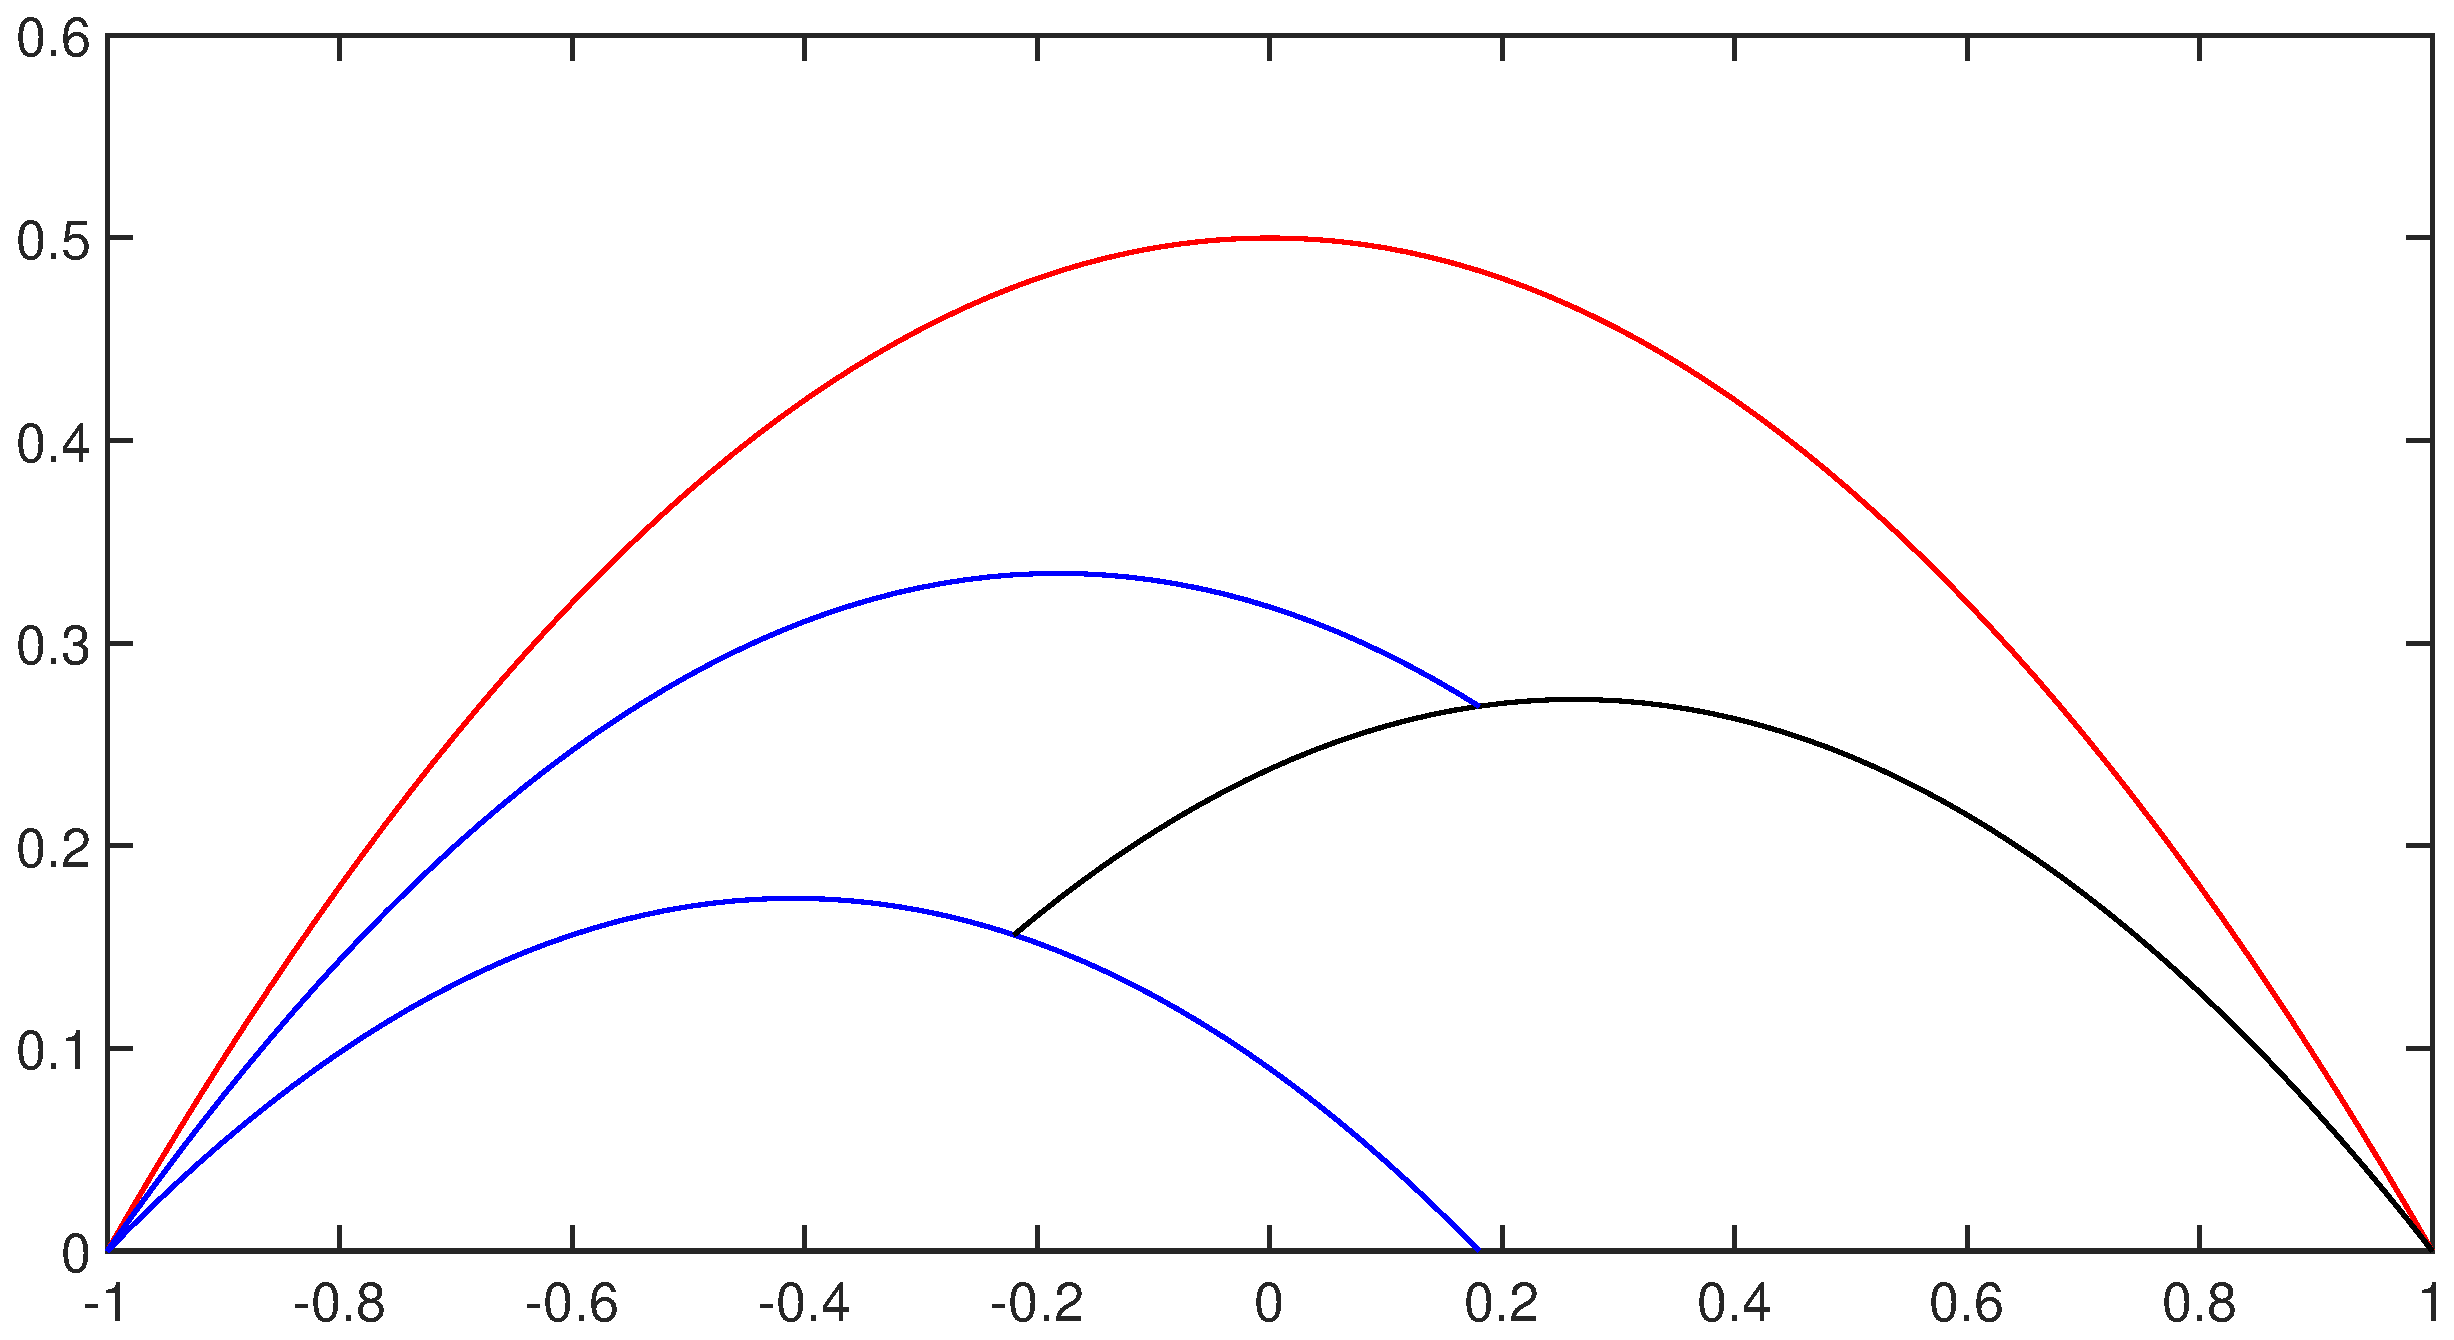
\includegraphics[width=\textwidth]{../AOSM/PLOT_SimpleSchwarz4.eps}}
	\only<5>{\includegraphics[width=\textwidth]{../AOSM/PLOT_SimpleSchwarz5.eps}}
\end{figure}
\end{frame}

\begin{frame}
\frametitle{Field-split Schwarz methods}

Instead of splitting up the physical domain, we can split up the problem into fields.

Suppose a problem can be written as
\begin{equation*}
	\begin{bmatrix} F(u,v) \\ G(u,v) \end{bmatrix} = \begin{bmatrix} f \\ g \end{bmatrix},
\end{equation*}
where $F$ depends more strongly on $u$ and $G$ depends more strongly on $v$.

Field-split multiplicative Schwarz:
\begin{equation*}
	F(u^{(n+1)},v^{(n)}) = f, \quad G(u^{(n+1)},v^{(n+1)}) = g.
\end{equation*}

\end{frame}

%% ASPIN/MSPIN/RASPEN
%\begin{frame}{Schwarz as a fixed point iteration}
%
%Schwarz methods can be represented as fixed point iterations:
%\begin{equation*}
%	u^{n+1} = g \left ( u^{n-1} \right ),
%\end{equation*}
%where $g(u)$ represents one iteration of a Schwarz method that takes boundary data from the input $u$.
%
%The fixed point of $g$ is the solution on the first subdomain.
%This is also the root of the function $f(u) = g(u) - u$.
%We apply Newton's method:
%\begin{equation*}
%	u^* = u^{n-1} - J(u^{n-1})^{-1} f(u^{n-1}),
%\end{equation*}
%where $J$ is the Jacobian of the function $f$.
%\end{frame}
%
%\begin{frame}{Schwarz-Preconditioned Newton methods (Cai \& Keyes, 2001)}
%
%This is equivalent to preconditioning Newton's method with a Schwarz method.
%
%Let
%\begin{equation*}
%	f(u) = \begin{bmatrix} f_1(u_1, u_2) \\ f_2(u_1,u_2) \end{bmatrix}.
%\end{equation*}
%Then Newton's method tells us to solve the nonlinear problem
%\begin{equation*}
%	\begin{bmatrix} J_{11}^{(n+1)} & J_{12}^{(n+1)} \\ J_{21}^{(n+1)} & J_{22}^{(n+1)} \end{bmatrix} \begin{bmatrix} u_1^{n+1} - u_1^n \\ u_2^{n+1} - u_2^n \end{bmatrix} = \begin{bmatrix} f_1 \\ f_2 \end{bmatrix},
%\end{equation*}
%where $J_{ij}^{(n+1)}$ is the derivative of $f_i$ with respect to $u_j$ evaluated at $u_1^{n+1}$ and $u_2^{n+1}$.
%\end{frame}
%
%\begin{frame}{Schwarz-Preconditioned Newton methods (Cai \& Keyes, 2001)}
%
%Preconditioning this with a parallel Schwarz method tells us to solve
%\begin{equation*}
%	\begin{bmatrix} J_{11}^{(n+1)} \\ & J_{22}^{(n+1)} \end{bmatrix} \begin{bmatrix} u_1^{n+1} - u_1^n \\ u_2^{n+1} - u_2^n \end{bmatrix} = \begin{bmatrix} f_1 \\ f_2 \end{bmatrix} - \begin{bmatrix} & J_{12}^{(n)} \\ J_{21}^{(n)} \end{bmatrix} \begin{bmatrix} u_1^{n} - u_1^{n-1} \\ u_2^{n} - u_2^{n-1} \end{bmatrix},
%\end{equation*}
%and completing the iteration by solving
%\begin{equation*}
%	\begin{bmatrix} J_{11}^{(n+1)} \\ & J_{22}^{(n+1)} \end{bmatrix}^{-1} \begin{bmatrix} J_{11}^{(n+1)} & J_{12}^{(n+1)} \\ J_{21}^{(n+1)} & J_{22}^{(n+1)} \end{bmatrix} \begin{bmatrix} u_1^* - u_1^n \\ u_2^* - u_2^n \end{bmatrix}
%	= \begin{bmatrix} f_1(u_1^{n+1},u_2^{n+1}) \\ f_2(u_1^{n+1},u_2^{n+1}) \end{bmatrix}.
%\end{equation*}
%
%\end{frame}

\section{Phasefield fracture and Newton-Schwarz} % 15 min

% phasefield
\begin{frame}{Brittle fracture}

\begin{figure}
\includegraphics[width=0.8\textwidth]{FIG/BrittleFracture.png}
\caption{Crack propagation in brittle material, image taken from paper by Blaise Bourdin} % nb: cite?
\end{figure}
\end{frame}

% phase-field fracture model
\begin{frame}{Phasefield fracture model}

\begin{equation*}
	E_\ell(u,\alpha) = \int \frac{1}{2} (1 - \alpha)^2 A e(u) \cdot e(u) dx + \frac{G_c}{4 c_w} \int \frac{w(\alpha)}{\ell} + \ell \abs{\nabla \alpha}^2 dx
\end{equation*}
\begin{itemize}
\item $u$ is a vector field which defines the displacement
\item $\alpha$ is a scalar field that is 0 away from the crack and 1 on the crack
\item $e(u)$ is the strain tensor, $A$ the stiffness tensor
\item $\ell$ determines the accuracy of the approximation of the Hausdorff measure of the crack
\item $w(0)=0$, $w(1)=1$, $w'(x) \geq 0$, $w \in C^1(0,1)$, $c_w = \int_0^1 \sqrt{w(s)} ds$
\item $G_c$ is the critical energy release rate
\item The model is quasi-static: energy is minimized for a given time step/external work, then the model steps forward in time
\end{itemize}
\end{frame}

\begin{frame}{Alternate minimization}

Cracks propagate to minimize $E_\ell(u,\alpha)$.
To model this, we then need to minimize over both $u$ and $\alpha$:
\begin{equation*}
	\begin{bmatrix} F(u,v) \\ G(u,v) \end{bmatrix} = \begin{bmatrix} \dx{}{u} E_\ell(u,\alpha) \\ \dx{}{\alpha} E_\ell(u,\alpha) \end{bmatrix} = \begin{bmatrix} 0 \\ 0 \end{bmatrix}.
\end{equation*}

The energy $E_\ell$ is not convex in both variables, but it is convex if either $u$ or $\alpha$ is kept constant.
This leads to alternate minimization.
\begin{algorithm}[H]
	\caption{Alternate Minimization (AltMin)}
	\begin{algorithmic}[1]
		\State Make initial guess $\alpha_0$ and set $n=0$
		\While{$\norm{\alpha_{n+1} - \alpha_n}$ is greater than tolerance}
			\State Find $u_{n+1} = \argmin_u E_\ell(u, \alpha_n)$
			\State Find $\alpha_{n+1} = \argmin_\alpha E_\ell(u_{n+1},\alpha)$
		\EndWhile
	\end{algorithmic}
\end{algorithm}
\href{PLOT_GD_AltMinAnimation.mp4}{\textcolor{blue}{(animation)}}
\end{frame}

% MSPIN
\begin{frame}{Applying Newton (Kopanicakova, Kothari \& Krause, 2023)}

AltMin can be thought of as a fixed point iteration over $\alpha$:
\begin{equation*}
	\alpha_{n+1} = \text{AltMin}(\alpha_n),
\end{equation*}
which stops when $\alpha_{n+1}$ is sufficiently close to $\alpha_n$.

To accelerate the otherwise linear convergence, we can apply Newton's method to AltMin($\alpha$) - $\alpha$ after line 4:
\begin{equation*}
	\begin{bmatrix} J_{uu} \\ J_{\alpha u} & J_{\alpha \alpha} \end{bmatrix}^{-1} \begin{bmatrix} J_{uu} & J_{u \alpha} \\ J_{\alpha u} & J_{\alpha \alpha} \end{bmatrix} \begin{bmatrix} u_* - u_n \\ \alpha_* - \alpha_n \end{bmatrix} = \begin{bmatrix} u_{n+1} - u_n \\ \alpha_{n+1} - \alpha_n \end{bmatrix},
\end{equation*}
where $J_{ij}$ is the second derivative of $E_\ell(u,\alpha)$ with respect to $i$ then $j$.

In practice, we solve this system inexactly and usually with some kind of backtracking to globalize Newton's method.
The resulting method is called multiplicative Schwarz preconditioning inexact Newton's method (MSPIN).
\end{frame}

\begin{frame}{Globalization techniques}

Newton's method needs globalization techniques to converge when the starting guess is far from a minimum.
The default choice is cubic backtracking:
\begin{algorithm}[H]
\caption{Cubic backtracking}
\begin{algorithmic}[1]
\State Inputs: current iterate $x_c$, search direction $p$, objective function $F(x)$
\State Set $\lambda_0 = 1$
\State Set $\lambda_1$ such that $x_p = x_c + \lambda_1 p$ minimizes the quadratic polynomial interpolating $F(x_c)$, $F(x_c + p)$ and $\nabla F(x_c)^\top p$
\While{$F(x_c + \lambda_1 p) \geq F(x_c)$ and $\norm{p} <$ some tolerance}
	\State Set $\lambda_2$ such that $x_c + \lambda_2 p$ minimizes the cubic polynomial interpolating $F(x_c)$, $F(x_c + \lambda_0 p)$, $F(x_c + \lambda_1 p)$ and $\nabla F(x_c)^\top p$
	\State $\lambda_0 \gets \lambda_1$, $\lambda_1 \gets \lambda_2$
\EndWhile
\end{algorithmic}
\end{algorithm}
\end{frame}

% parallelogram
\begin{frame}
\frametitle{Parallelogram minimization}

MSPIN is well-suited for a new kind of globalization technique because it requires finding two solutions for the same problem:
\begin{itemize}
\item the result from multiplicative Schwarz/AltMin, $x_c + q$, and;
\item the result from the Newton's method step, $x_c + p$.
\end{itemize}
This gives us two directions to look in, meaning we should seek our minimum in a parallelogram.

\centering
\begin{tikzpicture}
	\node[below left] at (0,0) {$x_c$};
	\node[below right] at (3,0) {$x_c + p$};
	\node[above left] at (1,2) {$x_c + q$};
	\node[above right] at (4,2) {$x_c + p + q$};
	\draw (0,0) -- (3,0) -- (4,2) -- (1,2) -- cycle;
\end{tikzpicture}

\end{frame}

\begin{frame}
\frametitle{Parallelogram minimization}

Given an objective function $F(x)$, minimize the polynomial $P(i,j) = ai^2 + b ij + cj^2 + d i + e j + f$, where
\begin{align*}
	f = & F(x_c),
	& e = & \nabla F(x_c)^\top p,
	& d = & \nabla F(x_c)^\top q,
	\\ c = & F(x_c + p) - e - f,
	& a = & F(x_c + q) - c - f,
\end{align*}
\begin{equation*}
	b = F(x_c + p + q) - F(x_c + p) - F(x_c + q) + f,
\end{equation*}
in the region where $0 < i, j < 1$.
\begin{equation*}
	\begin{bmatrix} i_{\text{min}} \\ j_{\text{min}} \end{bmatrix} \in \set{ \begin{bmatrix} \frac{-2cd + be}{4ac - b^2} \\ \frac{-2ae + bd}{4ac - b^2} \end{bmatrix}, 
	\begin{bmatrix} 0 \\ -\frac{e}{2c} \end{bmatrix}, \begin{bmatrix} -\frac{d}{2a} \\ 0 \end{bmatrix}, \begin{bmatrix} 1 \\ -\frac{e + b}{2c} \end{bmatrix}, \begin{bmatrix} -\frac{d + b}{2a} \\ 1 \end{bmatrix}, 
	\begin{bmatrix} 0 \\ 1 \end{bmatrix}, \begin{bmatrix} 1 \\ 0 \end{bmatrix}, \begin{bmatrix} 1 \\ 1 \end{bmatrix} }
\end{equation*}
\end{frame}

% nb: numerical results?

% nb: project proposal: analyze parallelogram minimization

\section{Adaptive optimized Schwarz methods}

\begin{frame}
\frametitle{More complicated DD example}
\begin{columns}
	\begin{column}{0.5\textwidth}
		\begin{figure}
			\centering
			\includegraphics[width=\textwidth]{FIG/Saad_airfoil.png}
			\caption{Airfoil from Saad's ``Iterative Methods''}
		\end{figure}
	\end{column}
	\begin{column}{0.5\textwidth}
		\begin{figure}
			\centering
			\includegraphics[width=\textwidth]{FIG/Saad_cover.png}
			\caption{Possible matrix for example}
		\end{figure}
	\end{column}
\end{columns}
\end{frame}

\begin{frame}
\frametitle{A general form of the matrix}

Let us consider matrices that can take the form
\begin{equation} \label{eq: lin sys}
	\begin{bmatrix}
		A_{11} & & & & A_{1 \Gamma} \\
		& A_{22} & & & A_{2 \Gamma} \\
		& & \ddots & & \vdots \\
		& & & A_{nn} & A_{n \Gamma} \\
		A_{\Gamma 1} & A_{\Gamma 2} & \dots & A_{\Gamma n} & A_{\Gamma \Gamma}
	\end{bmatrix}
	\begin{bmatrix} \vec{u}_1 \\ \vec{u}_2 \\ \vdots \\ \vec{u}_n \\ \vec{u}_\Gamma \end{bmatrix}
	=
	\begin{bmatrix} \vec{f}_1 \\ \vec{f}_2 \\ \vdots \\ \vec{f}_n \\ \vec{f}_\Gamma \end{bmatrix},
\end{equation}
where $A_{ii}$ are square.
This system represents $n$ subdomains connected through a global interface represented by $\Gamma$.

Each subdomain now has its own subproblem:
\begin{equation} \label{eq: subproblem}
	\begin{bmatrix}
		A_{ii} & A_{i \Gamma} \\
		A_{\Gamma i} & A_{\Gamma \Gamma} + S_i
	\end{bmatrix}
	\begin{bmatrix} \vec{u}_i \\ \vec{u}_\Gamma \end{bmatrix}
	=
	\begin{bmatrix} \vec{f}_i \\ \tilde{\vec{f}}_i \end{bmatrix},
\end{equation}
where $\tilde{\vec{f}}_i$ is some modification of $\vec{f}_\Gamma$,
and $S_i$ is some global transmission matrix.
%We see that the variables associated with the global interface $\Gamma$ appear in all subproblems.
%The global transmission matrix $S_i$ dictates how these many copies communicate with one another.
\end{frame}

\begin{frame}
\frametitle{How to choose $S_i$ and $\tilde{\vec{f}}_i$}

There are perfect choices of $S_i$ and $\tilde{\vec{f}}_i$ such that each subproblem gives the exact solution to the global problem on its respective subdomain.
However, these perfect choices are expensive to compute.

Instead, the standard procedure is to make \textit{a priori} choices that give convergent iterative methods.
These appear as:
\begin{equation} \label{eq: iterative sub}
	\begin{bmatrix}
		A_{ii} & A_{i \Gamma} \\
		A_{\Gamma i} & A_{\Gamma \Gamma} + S_i
	\end{bmatrix}
	\begin{bmatrix} \vec{u}_i^{(k+1)} \\ \vec{u}_{\Gamma i}^{(k+1)} \end{bmatrix}
	=
	\begin{bmatrix} \vec{f}_i \\ \vec{f}_\Gamma \end{bmatrix}
	+ \sum_{j \neq i}
	\begin{bmatrix} ~ \\ -A_{\Gamma j} & T_j \end{bmatrix}
	\begin{bmatrix} \vec{u}_j^{(k)} \\ \vec{u}_{\Gamma j}^{(k)} \end{bmatrix},
\end{equation}
where
\begin{equation} \label{eq: local to global transmission}
	S_i = \sum_{j \neq i} T_j.
\end{equation}
\end{frame}

\begin{frame}
\frametitle{Choices for $T_j$}

The local transmission matrices $T_j$ can represent boundary conditions between the subdomains.
Some common options:
\begin{itemize}
\item Dirichlet, setting the interface variables on connected subdomains to be the same
\item Neumann, setting the derivatives to be the same
\item Optimized, setting Robin boundary conditions to be the same, using a Robin parameter that optimizes convergence rates
\end{itemize}

The strategy we'll employ here is to adapt the transmission conditions at each iteration so that they're closer to the perfect choices.

\end{frame}

\begin{frame}
\frametitle{Symmetrized cells}

\begin{columns}
	\begin{column}{0.5\textwidth}
For each subdomain, take a copy of it and stitch it together along their shared interface.
This pair is now perfectly symmetric, and one subproblem describes both copies.

\begin{equation} \label{eq: sym cell}
	\begin{bmatrix}
		A_{ii} & A_{i \Gamma} \\
		A_{\Gamma i} & A_{\Gamma \Gamma} & A_{\Gamma i} \\
		& A_{i \Gamma} & A_{ii}
	\end{bmatrix}
	\begin{bmatrix} \hat{\vec{u}}_i \\ \hat{\vec{u}}_\Gamma \\ \hat{\vec{u}}_i \end{bmatrix}
	=
	\begin{bmatrix} \vec{f}_i \\ \hat{\vec{f}}_i \\ \vec{f}_i \end{bmatrix}.
\end{equation}
	\end{column}

\tdplotsetmaincoords{60}{110}
\def\SplitAngle{120}
\def\AngleSplit{300}
	\begin{column}{0.5\textwidth}
\begin{figure}
	\begin{tikzpicture}[tdplot_main_coords]
		\fill[left color=blue!50] (180:1 and 1) arc (180:\AngleSplit:1 and 1) -- ++(0,0,2) arc (\AngleSplit:180:1 and 1) -- cycle;
		\fill[left color=blue!50] (1,0,0) arc (360:\AngleSplit:1 and 1) -- ++(0,0,2) arc (\AngleSplit:360:1 and 1) -- cycle;
		\foreach \x in {-2,...,2} {
			\draw[gray, thin] (\x,0,-1) -- (\x,0,3);
		}
		\foreach \z in {-1,...,3} {
			\draw[gray, thin] (-2,0,\z) -- (2,0,\z);
		}
		\fill[right color=red!10] (\SplitAngle:1 and 1) arc (\SplitAngle:180:1 and 1) -- ++(0,0,2) arc (180:\SplitAngle:1 and 1) -- cycle;
		\fill[right color=red!10] (1,0,0) arc (0:\SplitAngle:1 and 1) -- ++(0,0,2) arc (\SplitAngle:0:1 and 1) -- cycle;
	\end{tikzpicture}
	\caption{A symmetrized square domain with interfaces on two opposing edges}
\end{figure}
	\end{column}
\end{columns}
\end{frame}

\begin{frame}
\frametitle{Adaptive optimized Schwarz on symmetrized cells}

We solve the following iterations to correct the initial solution:
\begin{equation} \label{eq: sym cells AOSM}
	\begin{bmatrix}
		A_{ii} & A_{i \Gamma} \\
		A_{\Gamma i} & A_{\Gamma \Gamma} + T_i^{(k+1)}
	\end{bmatrix}
	\begin{bmatrix} \vec{d}_i^{(k+1)} \\ \vec{d}_{\Gamma i}^{(k+1)} \end{bmatrix}
	=
	\begin{bmatrix} ~ \\ -A_{\Gamma i} & T_i^{(k)} \end{bmatrix}
	\begin{bmatrix} \vec{d}_i^{(k)} \\ \vec{d}_{\Gamma i}^{(k)} \end{bmatrix},
\end{equation}
where $\vec{d}_i^{(k+1)} = \vec{u}_i^{(k+1)} - \vec{u}_i^{(k)}$.

We can use techniques from static condensation to reduce the form of this system to acting only on the global interface:
\begin{equation} \label{eq: static}
	\left ( \hat{A}_i + E_i^{(k+1)} \right ) \vec{d}_{\Gamma i}^{(k+1)} = E_i^{(k)} \vec{d}_{\Gamma i}^{(k)},
\end{equation}
where
\begin{equation*}
	\hat{A}_i = A_{\Gamma \Gamma} - 2 A_{\Gamma i} A_{ii}^{-1} A_{i \Gamma}, \quad E_i^{(k)} = T_i^{(k)} + A_{\Gamma i} A_{ii}^{-1} A_{i \Gamma}.
\end{equation*}

\end{frame}

\begin{frame}
\frametitle{Updates to the transmission condition}

We have one input, $\vec{d}_{\Gamma i}^{(k)}$, and one output, $E_i^{(k)} \vec{d}_{\Gamma i}^{(k)}$.
This is enough to give a rank one approximation of $E_i^{(k)}$, which we can use to update the transmission conditions:
\begin{equation*}
	T_i^{(k+1)} := T_i^{(k)} - E_i^{(k)} \frac{\vec{d}_{\Gamma i}^{(k)} \left ( \vec{d}_{\Gamma i}^{(k)} \right )^\top}{\norm{\vec{d}_{\Gamma i}^{(k)}}^2}.
\end{equation*}

For subsequent iterations, we have to orthogonalize the vectors $\vec{d}_{\Gamma i}^{(k)}$:
	\begin{algorithmic}[1]
		\State Inputs: $\vec{d}_{\Gamma i}^{(k)}$, $E_i^{(k)} \vec{d}_{\Gamma i}^{(k)}$, all previous $\vec{d}_{\Gamma i}^{(j)}$ and $E_i^{(j)} \vec{d}_{\Gamma i}^{(j)}$
		\State Set $\vec{w}_k := \vec{d}_{\Gamma i}^{(k)}$ and $\vec{v}_k := E_i^{(k)} \vec{d}_{\Gamma i}^{(k)}$
		\For{$j=1:k-1$}
			\State $h \gets \langle \vec{d}_{\Gamma i}^{(j)}, \vec{w}_k \rangle$, $\vec{w}_k \gets \vec{w}_k - h \vec{d}_{\Gamma i}^{(j)}$
			\State $\vec{v}_k \gets \vec{v}_k - h \vec{v}_j$ % nb: I think this line is unnecessary since E_i^{(k)} has d^{(j)} in its null space
		\EndFor
		\State Output: $E_i^{(k+1)} := E_i^{(k)} - \vec{v}_k \vec{w}_k^\top$
	\end{algorithmic}
\end{frame}

\begin{frame}
\frametitle{Equivalence to a Krylov subspace method}

From static condensation \eqref{eq: static} we have that the vectors $\vec{d}_{\Gamma i}^{(k)}$ form a Krylov subspace:
\begin{equation*}
	\vec{d}_{\Gamma i}^{(k)} \in \mathcal{K}_k \left ( \left ( \hat{A}_i + E_i^{(1)} \right )^{-1} E_i^{(1)}, \vec{d}_{\Gamma i}^{(1)} \right ) = \mathcal{K}_k.
\end{equation*}
% mention or prove that this space doesn't change when updating T?

By solving the system \eqref{eq: sym cells AOSM} the vector $\vec{d}_{\Gamma i}^{(k+1)}$ is equal to
\begin{equation*}
	\vec{d}_{\Gamma i}^{(k+1)} = \left ( \hat{A}_i + E_i^{(k)} \right )^{-1} E_i^{(k)} \vec{x},
\end{equation*}
where $\vec{x} \in \mathcal{K}_k$ such that
\begin{align*}
	\left ( I -  \left ( \hat{A}_i + E_i^{(1)} \right )^{-1} E_i^{(1)} \right ) \left ( \vec{u}_{\Gamma i}^{(k-1)} + \vec{x} \right ) & \\
	- \left ( \hat{A}_i + E_i^{(1)} \right )^{-1} \left ( \vec{f}_\Gamma - 2 A_{\Gamma i} A_i^{-1} \vec{f}_i \right ) & \perp \mathcal{K}_k.
\end{align*}
This is a Galerkin condition on the pre-image of the next difference.
\end{frame}

\begin{frame}
\frametitle{AOSM is equivalent to FOM}

\begin{block}{Equivalence theorem of AOSM for general matrices, CM. (2025)}
The AOSM is equivalent to the full orthogonalization method (FOM).
\end{block}

FOM is a precursor to the generalized minimal residual method (GMRES), considered by some the default iterative method for solving asymmetric linear systems.

By adding in a small least squares problem to the AOSM to correct the vectors $\vec{d}_{\Gamma i}^{(k)}$ and $\vec{d}_i^{(k)}$, we can get equivalence to GMRES.
This would minimize the residual within the Krylov subspace at each iteration.
\end{frame}

\begin{frame}
\frametitle{Convergence of the AOSM}

Because of the equivalence to FOM (and FOM's relations to GMRES), we can use the research there to tell us how AOSM will converge.
Unfortunately, that research tells us we can't know anything \textit{a priori}:
\begin{block}{Greenbaum, Ptak and Strakos (1996)}
Given a non-increasing positive sequence $\set{f_i}$ of real numbers and an arbitrary set of eigenvalues, there exists a matrix $A$ with these eigenvalues and a vector $\vec{b}$ such that the sequence of residuals of GMRES applied to the linear system $A \vec{x} = \vec{b}$ has norms equal to $\set{f_i}$.
\end{block}

Recent work has brought us closer to understanding the convergence properties of these methods. % nb: cite?
One project I propose is to build on this work in the specific context of Schwarz-preconditioned systems.

\end{frame}

\begin{frame}
\frametitle{Project proposal: AOSM/GMRES convergence}

\textbf{Project idea:} Investigate the convergence of GMRES and FOM by applying recent analysis methods to Schwarz-preconditioned systems.
Also study known worst-case convergence curves and if preconditioning techniques can improve rates.

\textbf{Possible collaborations:} Currently proposed as a postdoctoral project with Chen Greif (UBC) and Manfred Trummer (SFU), could also involve % nb: Yves, maybe Diane?

\textbf{Mentoring opportunities:} Studying GMRES convergence curves makes for a great PhD project.
The problem is well known in the community and any progress on it would make for an impressive thesis.

\end{frame}

% CG variant
\begin{frame}
\frametitle{AOSM on symmetric matrices}

When the matrix is symmetric, the target transmission conditions are as well.
Starting from a symmetric guess, the matrix $E_i^{(1)}$ will be also.

We want to choose updates that preserve symmetry:
\begin{equation*}
	T_i^{(k+1)} := T_i^{(k)} - \frac{\vec{v}_k \vec{v}_k^\top}{\vec{v}_k^\top \vec{w}_k}.
\end{equation*}

The orthogonalization is now with respect to an A-norm:
\begin{algorithmic}[1]
\State Inputs: $\vec{d}_{\Gamma i}^{(k)}$, $E_i^{(k)} \vec{d}_{\Gamma i}^{(k)}$, all previous $\vec{d}_{\Gamma i}^{(j)}$ and $E_i^{(j)} \vec{d}_{\Gamma i}^{(j)}$
\State Set $\vec{w}_k := \vec{d}_{\Gamma i}^{(k)}$ and $\vec{v}_k := E_i^{(k)} \vec{d}_{\Gamma i}^{(k)}$
\For{j=1:k-1}
	\State $h \gets \langle \vec{w}_k, \vec{v}_j \rangle$
	\State $\vec{w}_k \gets \vec{w}_k - h \vec{w}_j/\vec{v}_j^\top \vec{w}_j$
	\State $\vec{v}_k \gets \vec{v}_k - h \vec{v}_j / \vec{v}_j^\top \vec{w}_j$
\EndFor
\State Output: $E_i^{(k+1)} := E_i^{(k)} - \frac{\vec{v}_k \vec{v}_k^\top}{\vec{v}_k^\top \vec{w}_k}$
\end{algorithmic}
\end{frame}

\begin{frame}
\frametitle{Symmetric AOSM is equivalent to CG}

\begin{block}{Equivalence theorem of symmetric AOSM, CM. (preprint)}
The AOSM for symmetric matrices is equivalent to the conjugate gradient method (CG).
\end{block}

CG also minimizes an A-norm, but since the $A$ in question is symmetric, this is equivalent to minimizing the 2-norm. %nb: triple check this
Unlike for general matrices, the convergence properties of CG are known.
\begin{block}{Covnergence of AOSM for symmetric matrices}
The AOSM converges linearly and if the eigenvalues of $I -  \left ( \hat{A}_i + E_i^{(1)} \right )^{-1} E_i^{(1)}$ are clustered, then the AOSM converges superlinearly.
\end{block}

\end{frame}

\begin{frame}
\frametitle{Project proposal: AOSM versions of Krylov-Schwarz}

\textbf{Project idea:} Develop AOSM versions of existing Krylov subspace methods and compare against Krylov-Schwarz methods.
Also investigate best practices for size and shape of global interface, passing information between subdomains, and restricting global interface to local interface.

\textbf{Possible collaborations:} % nb: fill this out, maybe mention Felix and Martin

\textbf{Mentoring opportunities:} Modifications to an established algorithm would make for a good PhD project, and a straightforward introduction to high-performance computing.

\end{frame}

% numerical results: basic comparison with GMRES
\section{Numerical results of AOSM}

\begin{frame}{Simple comparison with other methods}

\begin{equation*}
	\begin{cases} \Delta u(x,y) = f(x,y), & (x,y) \in \Omega = [-1,1] \times [-1,1], \\
		u(x,y) = g(x,y), & (x,y) \in \partial \Omega. % = \set{x=-1} \cup \set{x=1} \cup \set{y=-1} \cup \set{y=1} .
	\end{cases}
\end{equation*}

\begin{figure}
	\begin{columns}
	\column{0.6\linewidth}
	\begin{tikzpicture}
			\draw[step=1em,red] (0,0) grid (5em,10em);
			\draw[step=1em,blue] (5em,0) grid (10em,10em);
			\node[below] at (5em,0) {$x_\Gamma$};
			\draw[very thick, black] (5em,0) -- (5em,10em);
			\node[above] at (5em,10em) {$\Omega$};
			\draw[decorate,decoration={brace, amplitude=1em, raise=0.5em}] (0,0) -- (0,10em) node[midway, xshift=-2.5em] {100};
			\draw[decorate, decoration={brace, amplitude=0.5em, mirror, raise=0.5em}] (0,0) -- (4em,0) node[midway, yshift=-2em] {49};
			\draw[decorate, decoration={brace, amplitude=0.5em, mirror, raise=0.5em}] (6em,0) -- (10em,0) node[midway, yshift=-2em] {50};
	\end{tikzpicture}
	\column{0.3\linewidth}
	\caption{$100 \times 100$ evenly spaced grid split into two subdomains along the 50th value of $x$}
	\end{columns}
\end{figure}
\end{frame}

\begin{frame}{Simple comparison with other methods}
\begin{figure}
	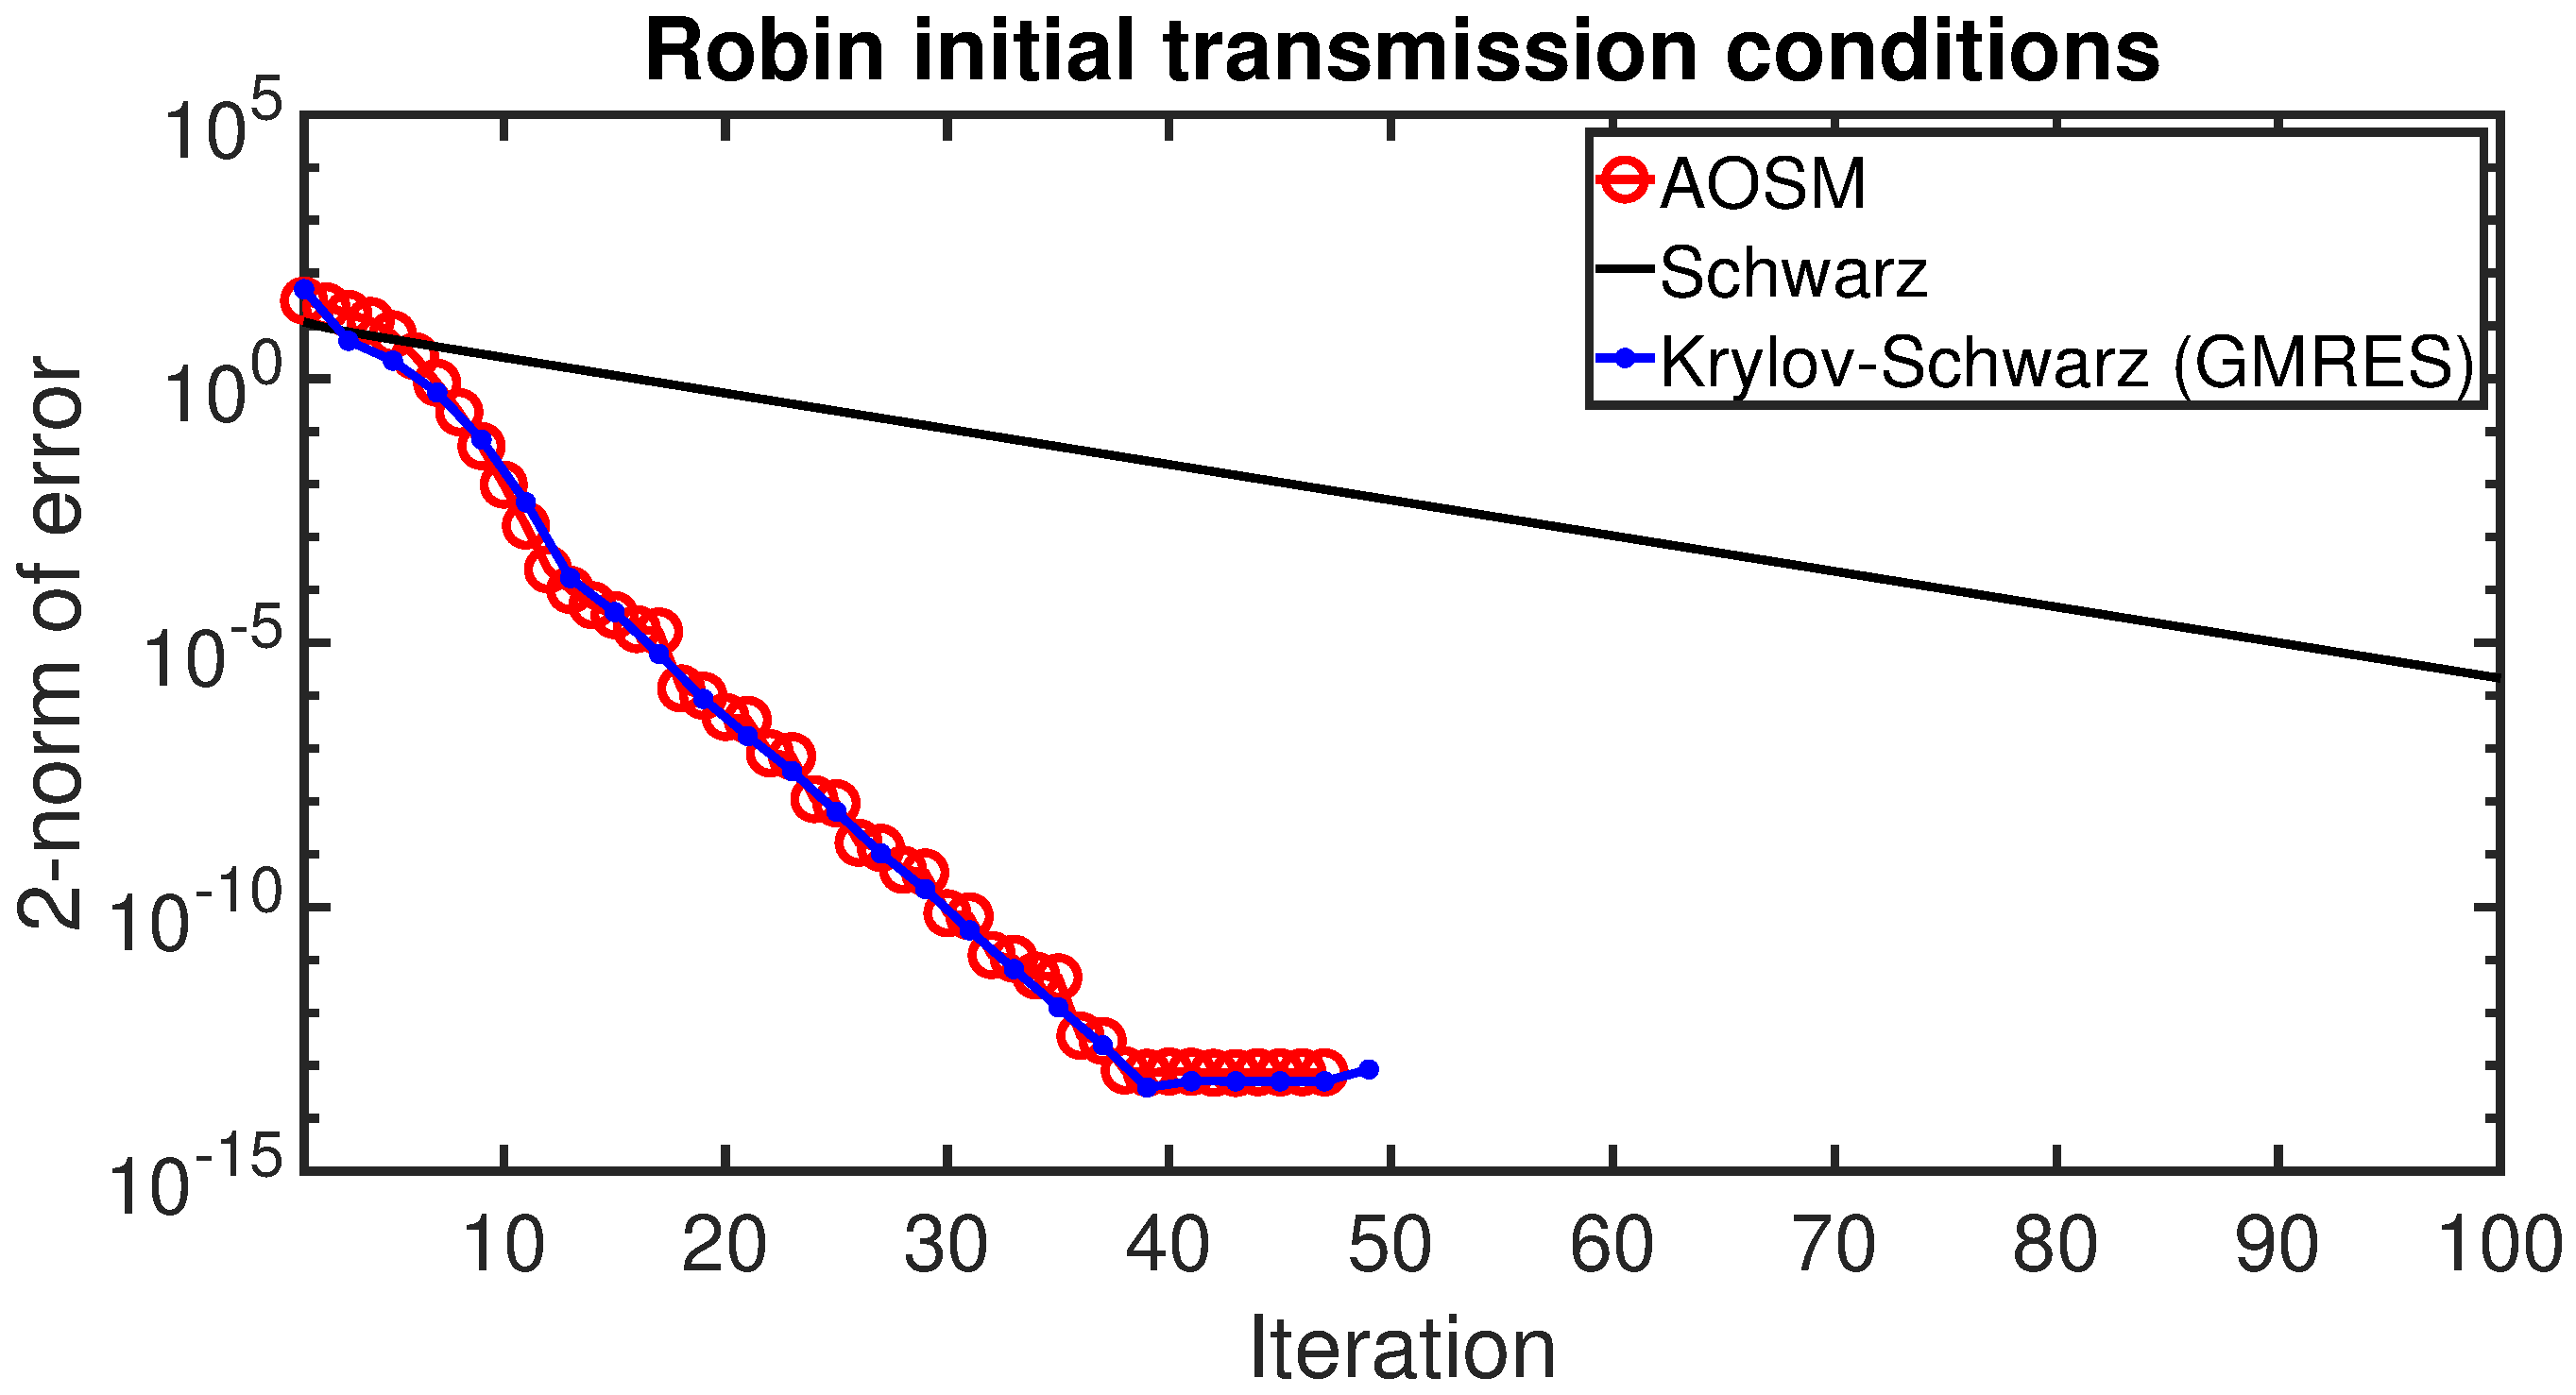
\includegraphics[width=\textwidth]{../AOSM/PLOT_faltAOSMConv_Seminar1.eps}
	\caption{Comparison between Schwarz, AOSM and Krylov-Schwarz on simple elliptic PDE}
\end{figure}
\end{frame}

% multiple subdomains (Schur complements for red-black)
\begin{frame}[fragile]
\frametitle{Precursor to multiple subdomains: red-black decompositions}
\begin{figure}
	\centering
	\begin{tikzpicture}
		\matrix[row sep=1em, column sep=1em]{%, ampersand replacement=\amp]{
			\draw[step=1em,red] (0,0) grid (3em,10em);
			\draw[step=1em,blue] (3em,0) grid (5em,10em);
			\draw[step=1em,red] (5em,0em) grid (7em,10em);
			\draw[step=1em,blue] (7em,0em) grid (10em,10em);
			\node[below] at (3em,0) {$x_\Gamma$};
			\draw[very thick, black] (3em,0) -- (3em,10em);
			\node[below] at (5em,0) {$x_\Gamma$};
			\draw[very thick, black] (5em,0) -- (5em,10em);
			\node[below] at (7em,0) {$x_\Gamma$};
			\draw[very thick, black] (7em,0) -- (7em,10em);
			\node[above] at (5em,10em) {$\Omega$};
			& \draw[thick,black,->] (0,5em) -- (0.5,5em); &
			\draw[step=1em,red] (0,0) grid (3em,10em);
			\draw[step=1em,red] (5em,0em) grid (7em,10em);
			\node[above] at (5em,10em) {$\Omega_1$}; &
			\draw[step=1em,blue] (3em,0) grid (5em,10em);
			\draw[step=1em,blue] (7em,0em) grid (10em,10em);
			\node[above] at (5em,10em) {$\Omega_2$};
		\\};
	\end{tikzpicture}
	\caption{Splitting the $100 \times 100$ grid into four strips, then pairing the strips into two algebraic subdomains}
\end{figure}
\end{frame}

\begin{frame}{Comparison: stripwise}
\begin{figure}
	\centering
	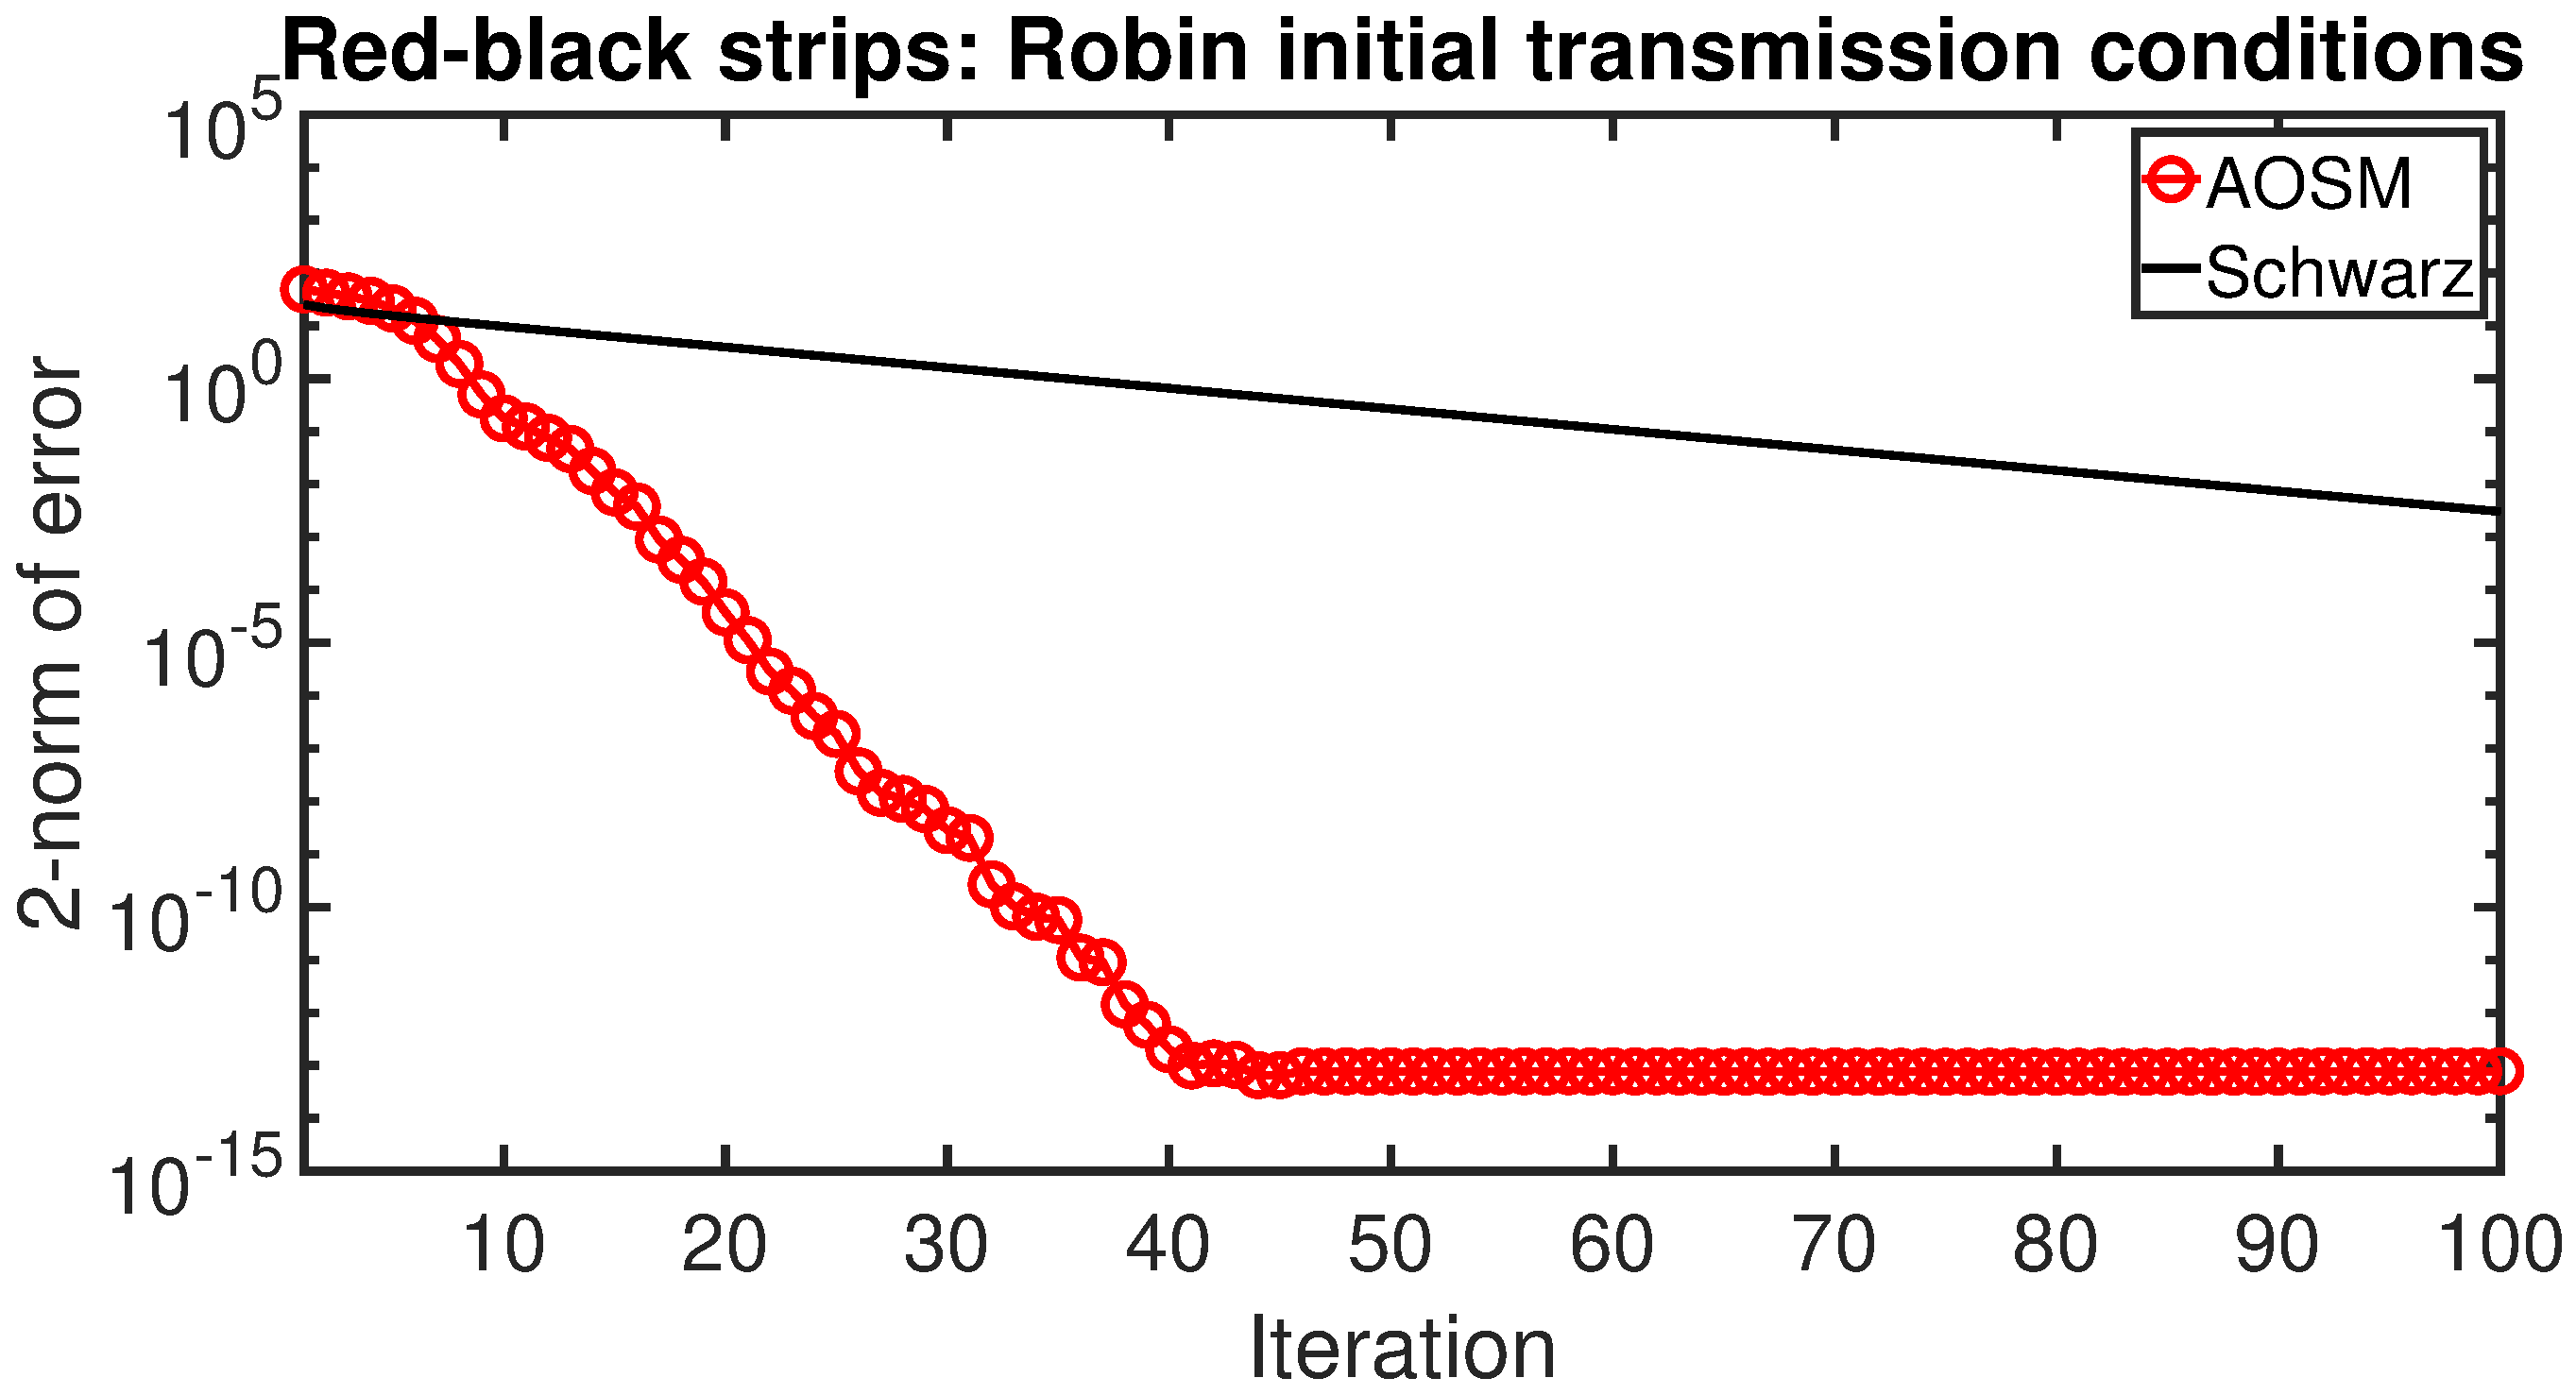
\includegraphics[width=\textwidth]{../AOSM/PLOT_RedBlack_Seminar2.eps}
	\caption{Convergence for AOSM and Schwarz on the stripwise decomposition}
\end{figure}
\end{frame}

\begin{frame}{Adapted transmission conditions: stripwise}
\begin{figure}
	\centering
	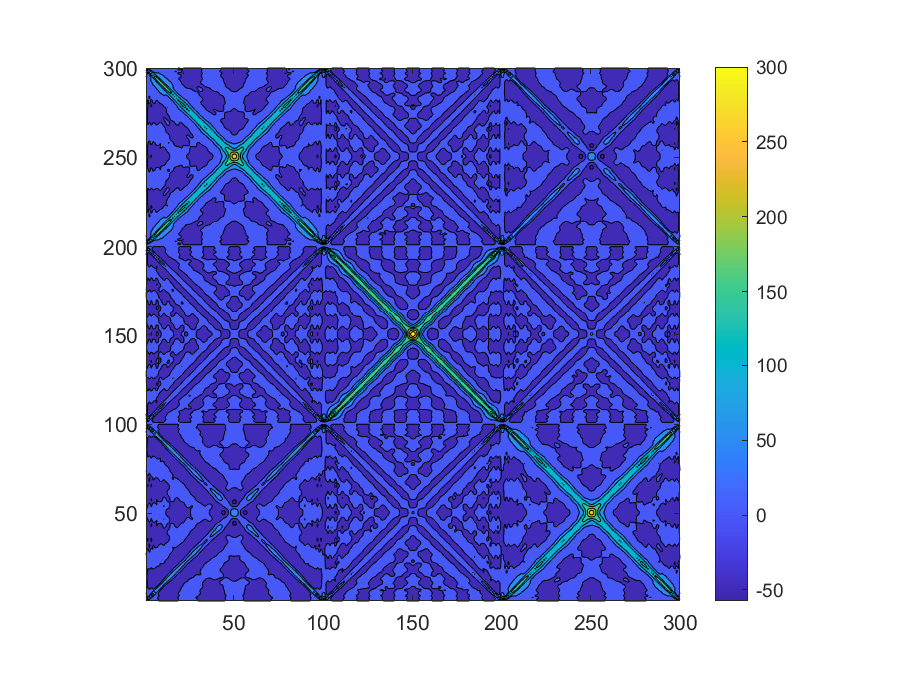
\includegraphics[width=0.8\textwidth]{../AOSM/PLOT_RedBlack_T_Seminar3.eps}
	\caption{Matrix $T_{1 \to 2}$ from AOSM after convergence of stripwise example}
\end{figure}
\end{frame}

\begin{frame}{Heterogeneous elliptic PDE}
\begin{equation*}
	\begin{cases} -\nabla \left ( \alpha(x,y) \cdot \nabla u(x,y) \right ) = f(x,y), & (x,y) \in \Omega = [0,1] \times [0,1], \\
		u(x,y) = g(x,y), & (x,y) \in \partial \Omega. % = \set{x=-1} \cup \set{x=1} \cup \set{y=-1} \cup \set{y=1} .
	\end{cases}
\end{equation*}

\begin{figure}
	\begin{columns}
	\column{0.6\linewidth}
	\centering
	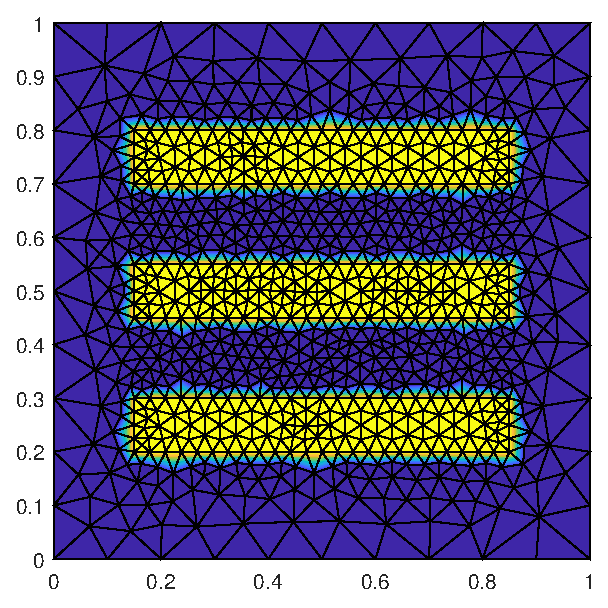
\includegraphics[height=0.6\textheight]{../AOSM/PLOT_LonelandK_Seminar.eps}
	\column{0.3\linewidth}
	\caption{$\alpha(x,y)=1$ except along three thin channels where $\alpha(x,y)=1000$}
	\end{columns}
\end{figure}
\end{frame}

\begin{frame}{Unstructured grid}
\begin{figure}
	\begin{columns}
	\column{0.6\linewidth}
	\centering
	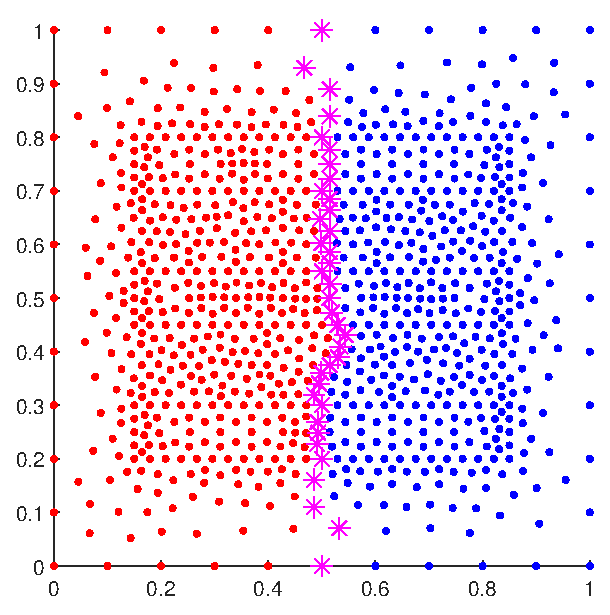
\includegraphics[height=0.6\textheight]{../AOSM/PLOT_LonelandSubdomains_Seminar.eps}
	\column{0.3\linewidth}
	\caption{Splitting an unstructured grid into two subdomains}
	\end{columns}
\end{figure}
\end{frame}

\begin{frame}{First round of solves}
\begin{figure}
	\centering
	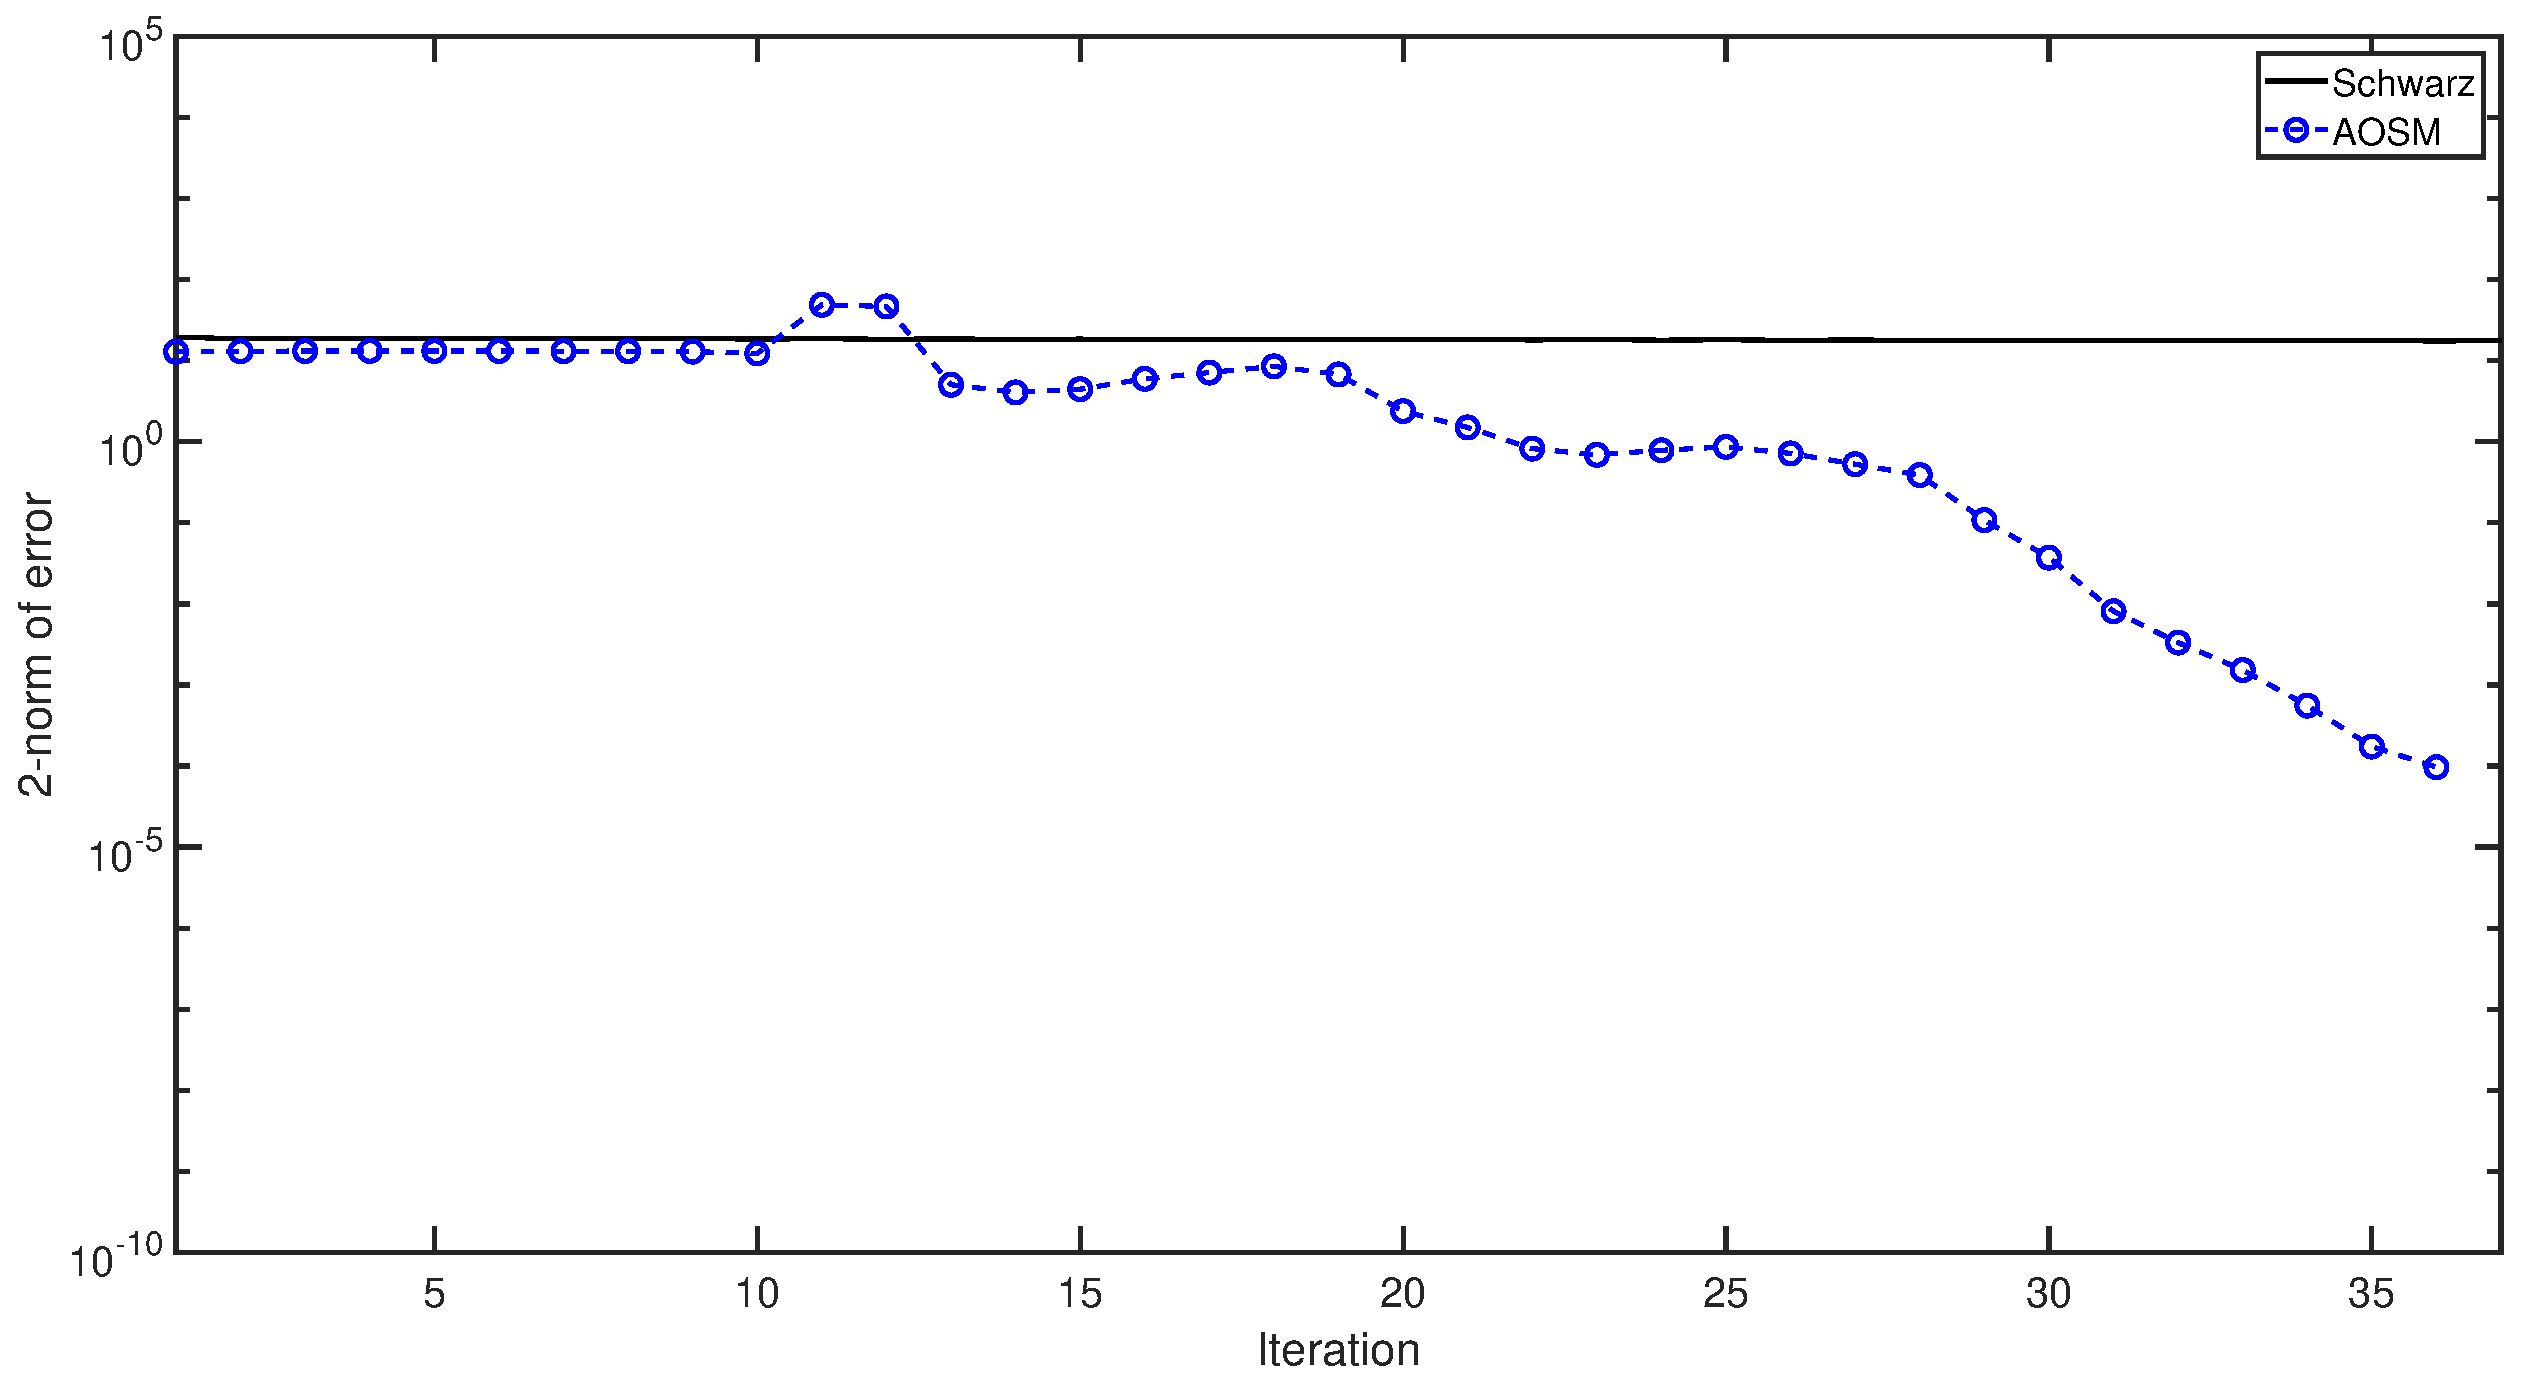
\includegraphics[width=\textwidth]{../AOSM/PLOT_LonelandFirst_Seminar.eps}
	\caption{(Lack of) convergence for Schwarz and AOSM for heterogeneous elliptic PDE}
\end{figure}
\end{frame}

\begin{frame}{Second round of solves}
\begin{figure}
	\centering
	\includegraphics[width=\textwidth]{../AOSM/PLOT_LonelandSecond_Seminar.eps}
	\caption{Convergence for Schwarz and AOSM using adapted transmission conditions}
\end{figure}
\end{frame}

\end{document}